\chapter{High Level Toolflow}
%Summary: Introduce idea of end to end toolflow
%Goal: Defend the idea that we can design an instrument using only a simple high level specification
%1
%State: Can be partially written now
%The end description will likely change based on the partitioning results

%Summary: describe CASPER, PASP and reconfigurable heterogeneous setispec Goals:
%describe the existence and continued development of �blocks�
%show the ability to design reconfigurable instruments by adding a layer of abstraction to the CASPER+xgpu work
%State: Can be written now
%Content already exists in the form of talks and a short paper.


%TODO: This will likely be moved elsewhere, including it here temporarily
\section{Instrument Generation}

%From USRI 2011 paper
Automatic Generation of Heterogeneous Spectrometers for Radio Astronomy

We have developed a software package to automatically generate spectrometers with minimal user input.
Spectrometer design is often done by building the instrument from scratch.
We have automated this design, creating a parameterized spectrometer that only requires a recompile to implement a change in specification.
This spectrometer combines FPGAs and GPUs, doing coarse channelization on the FPGA and sending each subband to the GPUs for further processing.
The server software is designed for flexibility, allowing astronomers to easily modify the processing algorithm run on the GPU and customize the instrument to fit their science goals.

\section{Introduction}
The need for high bandwidth spectroscopy manifests in many different radio astronomy applications.
Keeping up with increasing computation demands has often resulted in the specialized design of spectrometers.
At the Collaboration for Astronomy Signal Processing and Electronics Research (CASPER), we have developed a software package to automatically generate spectrometers for a variety of applications.

The CASPER FPGA libraries were developed to mitigate the need to redevelop common signal processing blocks for every new instrument \cite{Parsons:2009vc}. 
Parameterized blocks such as FFTs and digital down-converters can easily be used to design many different instruments. 
Coupled with open source FPGA boards, such as the ROACH (Reconfigurable Open Architecture Computing Hardware), the CASPER libraries provide a useful toolbox for radio astronomy instrumentation development.
This work extends the CASPER philosophy, demonstrating that entire instruments can be generated with minimal user input.
Rather than designing a completely different instrument for every different specification, this software package is parameterized so a change in specification only requires a recompile.

The software package includes an FPGA design and server software to do spectroscopy, as well as server benchmarks used to determine an optimal instrument configuration.
%The benchmarks measure maximum amount of data the servers can process, determining the optimal configuration for the instrument.
Both the FPGA and server software are parameterized, allowing for rapid deployment of a working spectrometer that is configured to take full advantage of available computing resources.
%Our general purpose approach allows for the rapid development of new instruments.
We implement the instrument on a heterogeneous cluster consisting of both FPGAs and GPUs to take advantage of the benefits provided by both platforms.
FPGAs provide high bandwidth processing but can be cumbersome to program.
GPUs can't handle the same bandwidths as FPGAs but they are easier to program. 
The CUDA language, for example, is a C-like language that can be used to develop software for many GPUs.
The high level parameters in this package allow us to use FPGAs while abstracting away implementation details specific to the FPGA.
To give the user control over their data processing algorithm, an application specific GPU program can be written and easily interfaced with the existing receive software in the package.
%Heterogeneous clusters 

\section{Radio Astronomy Applications}
This instrument has a wide variety of potential applications due to the flexibility of the server software. 
In this section, we describe a few specific applications than can make use of this package.

In the search for extraterrestrial intelligence (SETI), the ability to keep up with changes in technology allows searching instrumentation to stay on the leading edge of sensitivity. 
SETI aims to process the maximum bandwidth possible with very high resolution spectroscopy.
This instrument allows SETI projects to easily keep up with improvements on the telescope and increasing computational power.
An increase in detector bandwidth, improving the breadth of the search, can be processed simply recompiling the FPGA design and distributing the extra subbands to new servers. 
As computation improves, the instrument can be reconfigured to send more bandwidth to each computer, reducing the required cluster size, or improve the resolution of the instrument by doing a larger FFT on the server.

This design also has applications in pulsar science. 
The fast channelization on the FPGA with no data reduction makes it an ideal pulsar spectrometer, since no information is lost before sending the data to the servers.
GPUs provide a good platform for pulsar processing algorithms such as coherent dedispersion \cite{Ransom:2009wz}, which can easily be used as the processing function for the server software distributed in our package. 
Similar to SETI instruments, pulsar instruments designed using this package can also keep up with improvements in technology with a simple recompile.


\section{Instrument Architecture}
The instruments generated with this package use a heterogeneous design, allowing us to benefit from the strengths of FPGAs and GPUs. 
The FPGA board is able to sample and process very high bandwidths that a single CPU or GPU would not be able to manage; 
once the FPGA has split up the band the GPU provides a platform that is easier than an FPGA to program but still provides high compute power. 
A design called the Packetized Astronomy Signal Processor, or PASP, is run on the FPGA.
PASP splits up the large band into smaller bands that can be processed using off the shelf servers.
The subbands are put into packets on the FPGA and sent over a 10 gigabit Ethernet switch to a cluster of servers.
The servers receive the data from the switch and process it using spectroscopy software provided in the software package or special purpose application software written by the user and linked into the provided packet processing infrastructure.

Figure \ref{fig:spec_highlevel} shows a high level view of a spectrometer that could be designed with this package. 
In this example, a ROACH board divides the input band into 64 subbands and sends them out to a 16 server cluster.
An ADC is used to digitize data from the telescope and connects to the ROACH board via Z-DOK connectors. 
The digitized data is split into 64 subbands and sent through a 10 gigabit Ethernet switch.
Each server in the cluster receives and processes 4 subbands.

\begin{figure}[ht!]
  \centering
     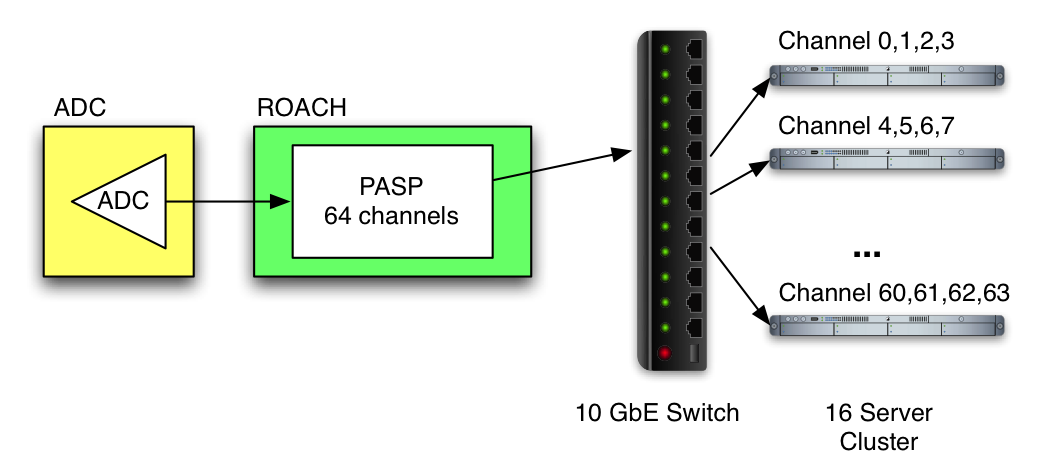
\includegraphics[width=1\textwidth]{Images/C4/spec_highlevel.png}
  \caption{Example high level instrument architecture}
  \label{fig:spec_highlevel}
\end{figure}


\subsection{FPGA Design}

%TODO : stuff about the pasp design here

Figure \ref{fig: pasp_fpga_arch} gives an overview of the dataflow through the FPGA.
The FPGA interfaces to a single ADC board that simultaneously digitizes 2 signals. 
Each signal can be sampled at a maximum rate of 1Msps.
The samples are sent into a polyphase filter bank (PFB), consisting of an FIR filter and an FFT, which breaks up the entire bandwidth sampled by the ADC into smaller subbands.
After dividing up the subbands, each band is rescaled. 
This step allows us to compensate for the shape of the analog filter feeding data into the ADC. 
After rescaling, the FPGA forms packets where each packet contains data from a single subband. %TODO fix
The packets are sent out over CX4 ports to a 10 gigabit Ethernet switch.

\begin{figure}[ht!]
  \centering
    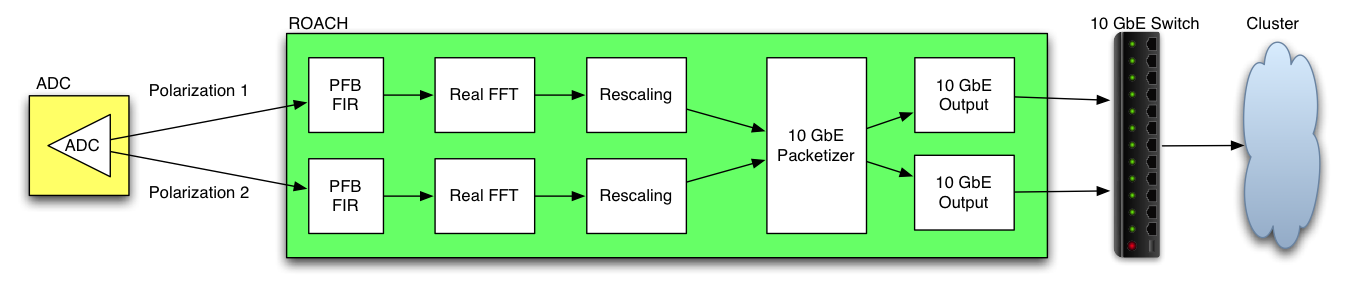
\includegraphics[width=1\textwidth]{Images/C4/pasp_fpga_arch.png}
  \caption{PASP Dataflow}
  \label{fig: pasp_fpga_arch}
\end{figure}

PASP uses a PFB to split up the subbands. Figure \ref{fig: fft_vs_pfb_response} shows a comparison between the FFT and PFB response. 
The FFT response (on the left) has a lot of spectral leakage while the PFB (on the right) has a much sharper filter shape and a better frequency response. 
The superior frequency response led us to use a PFB rather than an FFT to extract subbands, despite the additional FPGA resources required by the FIR filter before the FFT.

\begin{figure}[ht!]
  \centering
    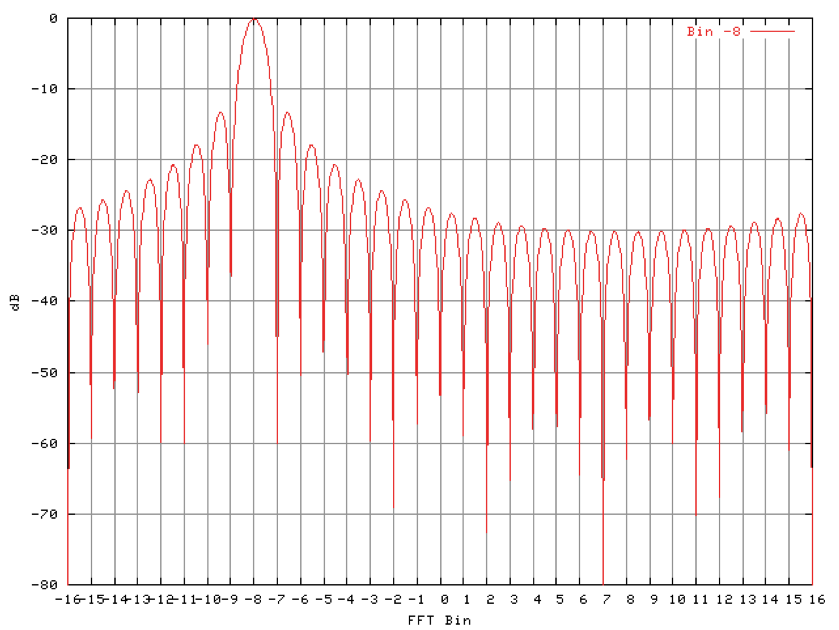
\includegraphics[width=0.48\textwidth]{Images/C4/fft_response.png}
    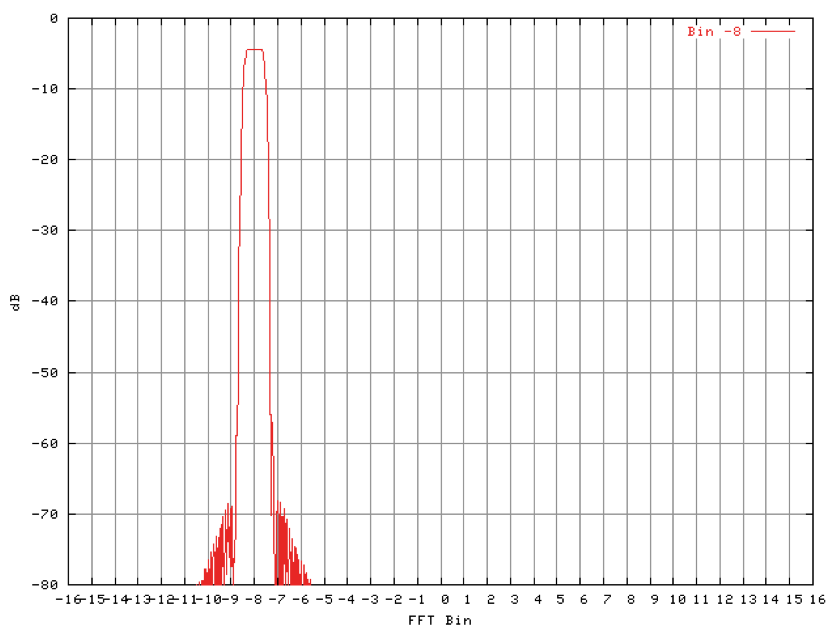
\includegraphics[width=0.48\textwidth]{Images/C4/pfb_response.png}
  \caption{A comparison of FFT and PFB response}
  \label{fig: fft_vs_pfb_response}
\end{figure}

PASP is designed for flexibility. 
Building on the CASPER goal to automate the design of commonly used signal processing elements such as FFTs and digital downconverters, PASP automatically designs an entire FPGA instrument using only a few parameters.
The user can input the desired number of subbands, CPU/GPU cluster size, and packet size and a new design is automatically generated in Simulink.  


\subsection{Server Benchmarking}
PASP has proven useful in many applications by itself, but the goal of automatically generating a spectrometer for any cluster requires more than just a reconfigurable FPGA design. 
It is difficult to determine what size the subbands or the cluster should be without knowing how much data the target servers can receive and process.
Our benchmarking tools are designed to quickly determine how much bandwidth a server is capable of handling so the PASP parameters can be set appropriately.

We have developed a general purpose benchmark to test the networking capability of a server. 
This test uses an FPGA design to generate 10 gigabit Ethernet packets and transmits them to the server under test.
The FPGA design has a runtime programable packet size and packet rate. 
The packet size is set to the largest size allowed by the server and the packet rate is initially set low and ramped up while the receive software running on the server checks for dropped packets.
By searching for the highest bandwidth with no dropped packets, we find the maximum allowable data rate where the server should reliably receive all the data.

%The processing capabilities must also be tested. 
While specific processing algorithms may vary between scientific applications, an FFT benchmark provides insight into possible processing requirements for a variety of radio astronomy applications.
We developed an FFT benchmark using CUFFT, the CUDA FFT library, which supports FFT of arbitrary sizes and allows them to be run in batches on the GPU. 
Our benchmark tests a variety of FFT sizes and batch sizes.
In general, we have found that running larger FFTs and batching many FFTs together is necessary to fully take advantage of the computing resources on GPU.
Running this benchmark allows us to determine the maximum bandwidth that can be processed with the available resources.

Using these benchmarks, we can see how much compute power is provided by the server and determine the parameters that need to be entered into PASP.
The benchmarks also allow us to identify potential bottlenecks by comparing the maximum bandwidth the server can receive to the maximum bandwidth the server can process.
If the system is upgraded to reduce bottlenecks, it is easy to retest the server and recompile a PASP design that takes advantage of the new resources.


\subsection{Server Software}
Our package includes spectroscopy software that interfaces with the PASP design.
This software receives data over an Ethernet port and transfers it from the CPU to the GPU. 
The GPU runs an FFT and then sends the data back to the CPU to be recorded.
The GPU software, like the GPU benchmark, uses the CUFFT library to run FFT. 
The FFT size depends on the desired resolution for a specific application and an efficient batch size can be determined by running the FFT benchmark to find the best batch size for the given FFT size.

The server software was designed so other applications could easily be implemented on the GPU without altering or rewriting the receive code that interprets the packet headers and transfers data to the GPU.
Once the data is on the GPU, the software calls a process function and passes it a pointer to the GPU data.
An initialization function is called before the data processing begins to do any setup needed by the processing function, and an corresponding destroy function cleans up once the processing is complete.
In the spectroscopy software included in the package, the initialization function creates the FFT plan, the processing function calls CUFFT, and the destroy function deletes the FFT plan.
Modifying the application run on the GPU simply requires a redefinition of these three functions.
Using this interface, we successfully replaced the CUFFT processing with software developed for SETI searches designed by Kondo et al. \cite{Kondo:2010uk}.

\section{Conclusion and Future Work}
In this paper, we describe a radio astronomy instrument that is easily reconfigured to suit a variety of applications.
Figure \ref{fig: universal_arch} shows how this style of instrument design can be extended to a heterogeneous cluster running multiple processing algorithms at the same time.
All of these algorithms require the data to be broken up into subbands before it can be processed by the server which can be done on the same FPGA. 
Using multicast packets, multiple servers can subscribe to the same subbands generated on by PASP and process them in different ways. 

\begin{figure}[ht!]
  \centering
    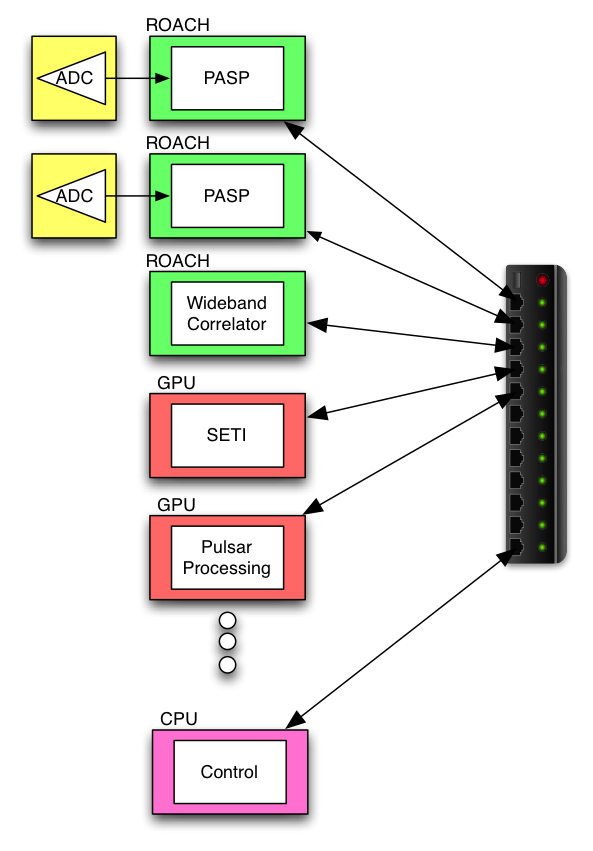
\includegraphics[width=0.5\textwidth]{Images/C4/universal_arch.png}
  \caption{A potential architecture for multiple scientific instruments simultaneously processing data from the same telescope}
  \label{fig: universal_arch}
\end{figure}

This style of instrument design greatly accelerates time to science for many projects.
Separating the implementation of the instrument from the hardware specification has created a design that works well for a variety of computational resources and applications.
As resources improve, the instrument can improve along with them, providing the opportunity to do new science that wasn't possible before.
